\documentclass[12pt]{article}
\usepackage{amsfonts, amssymb}
\usepackage{msc}
\usepackage{tikz}
	\usetikzlibrary{arrows, automata,positioning}
\usepackage{graphicx}
\usepackage{wrapfig}
\usepackage{float}
\usepackage{datetime}
\usepackage[ngerman]{babel}
\usepackage[utf8]{inputenc}
\usepackage{enumitem}
\usepackage{amsmath}
\usepackage{xspace}
\usepackage{multirow}
\usepackage{mathtools}
\usepackage{hyperref}

\newdateformat{specialdate}{\twodigit{\THEDAY}.\twodigit{\THEMONTH}.\THEYEAR}

\newcommand{\blue}[1]{\color{blue}#1\color{black}\xspace}
\newcommand{\red}[1]{\color{red}#1\color{black}\xspace}
\newcommand{\green}[1]{\color{green}#1\color{black}\xspace}

\makeatletter
\newcommand*\bigcdot{\mathpalette\bigcdot@{.5}}
\newcommand*\bigcdot@[2]{\mathbin{\vcenter{\hbox{\scalebox{#2}{$\m@th#1\bullet$}}}}}
\makeatother

\newcommand{\tabitem}{~~\llap{\textbullet}~~}

\begin{document}
	
	\title{MAO - Zusammenfassung}
	\author{Timo Bergerbusch}
	\date{\specialdate\today}
	\maketitle
	
	\tableofcontents
	\newpage
	
	\section{Typische Probleme} \label{Standard Probleme}
		\subsection{Matching}
			Paarbildung von adjazenten Knoten in einem ungerichteten bewerteten Graphen\\
			Matching $M$: jeder Knoten hat max. einen Partner Knoten\\
			perfektes Matching $M^*$: jeder Knoten hat genau einen Partner Knoten\\
			Optional: Kosten, Profite, etc\dots
		\subsection{Set-Packing/Covering/Partitioning}
			\subsubsection*{Gegeben: }
			\begin{itemize}
				\item $m$-elementige Menge $M={1, \dots, m}$
				\item $n$ Teilmengen $M_1,\dots,M_n \subset M$
				\item Kosten/Profite der Teilmengen $c_1,\dots,c_n$
			\end{itemize}
			\subsubsection*{Gesucht:} Auswahl von Teilmengen
			\begin{enumerate}
				\item mit max. Profit / min. Kosten
				\item die Grundmenge $M$ wird gepackt, überdeckt oder partitioniert
			\end{enumerate}			
			Eine Lösung $L$ ist ein
			\begin{itemize}
				\item Set-Packing, wenn $M_j \cap M_k = \emptyset \forall j,k \in L, j \neq k$
				\item Set-Covering, wenn $\bigcup_{j\in L} M_j = M$
				\item Set-Partitioning, wenn es sowohl Set-Packing als auch Set-Covering ist
			\end{itemize}
		\subsection{Traveling-Salesman-Problem (TSP)}\label{TSP}
			\subsubsection*{Gegeben:}
			\begin{itemize}
				\item vollständiger Graph $G=(V,E,d)$
				\item symmetrisch: $d_{i,j}=d_{j,i}\> \forall i,j\in V$
				\item asymmetrisch: $d_{i,j}\neq d_{j,i}\> \exists i,j \in V$
			\end{itemize}
			\subsubsection*{Gesucht:}
			kostenminimale Hamilton-Tour
			
			\subsubsection{Typische Distanzmatrixberechnung:}
			Euklidische Distanz: $d_{i,j}=\sqrt{(x_i-x_j)^2+(y_i-y_j)^2}$ \\
			Manhattan-Distanz: $d_{i,j}=|x_i-x_j|+|y_i+y_j|$
		\subsection{Bin-Packing-Problem (BPP)}
			\subsubsection*{Gegeben:}
				\begin{itemize}
					\item Kapazität $C>0$
					\item Gewichte $w_1,\dots,w_n$ mit $0<w_i\le C$
				\end{itemize}
			\subsubsection*{Gesucht:}
				Partitionierung $P_1\cup\dots\cup P_k = \{1,\dots,n\}$ mit $P_i\cap P_j = \emptyset$ und $\sum_{j\in P_i} w_j \le C$ für ein minimales $k$.

			\subsubsection*{Greedy-Algorithmus}\label{BPGreedy}
			Unterscheide die versch. Strategien
			\begin{itemize}
				\item Weight Decreasing: absteigend nach Gewicht sortiert
				\item Next-Fit: Zuordnung zum zuletzt geöffneten
				\item First-Fit: Zuordnung zumersten geöffneten Behälter mit kleinstem Index
				\item Best-Fit: Zuordnung zum Behälter mit kleinster noch ausreichender Kapazität
			\end{itemize}
		
		\subsection{Rucksackproblem (KP)}
			\subsubsection*{Gegeben:}
			\begin{itemize}
				\item Rucksack mit Kapazität $C$
				\item $n$ Gegenstände mit Gewicht $w_i$ und Profit $p_i$
			\end{itemize}
			
			\subsubsection*{Gesucht:}
			Profit-maximale Teilmenge von Gegenständen, welche nicht schwerer ist als $C$
			
			\subsubsection*{Greedy-Algorithmus}\label{KPGreedy}
			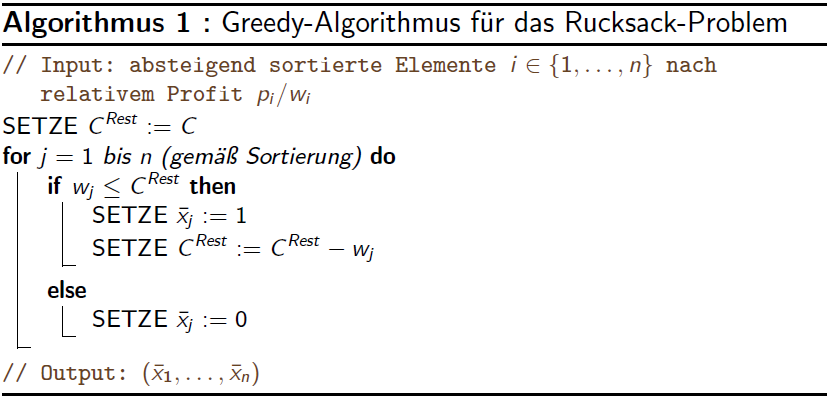
\includegraphics[scale=0.6]{KPGreedy}
	\section{1. Kapitel - Einführung}
	\begin{itemize}
		\item Abgrenzung Modell und Methode:
			\begin{itemize}
				\item[Modell:] modellieren, darstellen, abbilden
				\item[Methode:] rechnen, Algorithmus
			\end{itemize}
		\item Beispielanwendungen:
			\begin{itemize}
				\item Demand Planning: Welche Dienstleistungen auf welchen Flugstrecken
				\item Umlaufplanung: Welches Flugzeug für welchen Flug?
				\item Crew Scheduling: Wer erledigt wann welche Aufgaben?
				\item Disruption Management: Wie reagieren auf Störungen, Abweichungen und Ausfälle?
				\item Revenue Management: Pricing, Kapazitätssteuerung
				\item Netzwerk-Design: Welche Standorte und welche Aufgaben dort?
				\item Transportplanung
				\item Standort Planung
				\item "Letzte Meile": Bezirkseinteilung und Postbotenrouten
			\end{itemize}
		\item \textbf{optimal} \label{optimal}\label{Optimum}: zulässig und bestmöglich
		\item \textbf{Simulation} \label{Simulation}: Durchführung von Experimenten anhand von Modellen
		\item Optimierung:
			\begin{itemize}
				\item exakt vs. heuristisch
				\item kontinuierlich vs. diskret
				\item linear vs. nicht-linear 
			\end{itemize}
		\item \hyperref[Simulation]{Simulation} vs. Optimierung:
			\begin{itemize}
				\item Simulation zeigt nur Konsequenzen von Entscheidungen auf
				\item Simulation macht keinen Entscheidungsvorschlag
				\item Simulation gestattet nur den Vergleich von Alternativen
			\end{itemize}		
		\item \textbf{Heuristik} \label{Heuristik}: 
			\begin{itemize}
				\item[Def.:] Algorithmen die ein geg. Optimierungsproblem mit akzeptablem Aufwand in möglichst gut zu lösen versuchen
				\item[Kennzeichen:] Ausschluss potentieller Lösungen, fehlende Lösungsgarantie, nicht-willkürliche Lösungssuche(, künstliche Stoppregel)
				\item[Prinzipien] Allgemeinheit, Effizienz, Optimalität	\\
				\begin{tikzpicture}
				\node[rectangle, draw, rounded corners] (allg) {Allgemeinheit};
				\node[rectangle, draw, rounded corners, below right = 3cm of allg] (opt) {Optimalität};
				\node[rectangle, draw, rounded corners, above right = 3cm of opt] (eff) {Effizienz};
				
				\path[thick]
				(allg) edge node[sloped, align = left] {exaktes\\ Verfahren} (opt)
				(allg) edge node[anchor=south] {Heuristik} (eff)
				(opt) edge node[sloped, align = left] {Verfahren für \\ spez. Instanz} (eff);
				\end{tikzpicture}
				\item[Klassifikation] nach Stopp-Regel:
				\begin{enumerate}
					\item[Eröffnungsv.] generieren einer (mögl. guten) Lösung. Terminierung sobald Lösung gefunden
					\item[Verbesserungsv.] Start mit zulässiger Lösung und verbessern, bis Stopp-Krit. erfüllt ist
					\item[Zsm.-gesezte V.] Kombination von Eröffnungs- und Verbesserungsv.
				\end{enumerate} 
			\end{itemize}
		\item \textbf{Algorithmus} \label{Algorithmus}: 
			\begin{itemize}
				\item[Def.:] Ein Algorithmus ist eine genau definierte Verarbeitungsvorschrift zur Lösung eines Problems oder einer bestimmten Art von Problemen. Typischerweise wird ein Algorithmus durch eine endliche Folge von Anweisungen beschrieben, die nacheinander ausgeführt und oft in festgelegter Weise wiederholt werden
				\item[Eig.:] eindeutig, allgemein, ausführbar, endlich
			\end{itemize}
		\item \textbf{exakter Algorithmus} \label{exakter Algorithmus}: ein \hyperref[Algorithmus]{Algorithmus}, welcher für jede Instanz
			eines Optimierungsproblems ein \hyperref[Optimum]{Optimum} bestimmt
		\item \textbf{Laufzeitkomplexität}: \hyperref[Algorithmus]{Alg. A} ist in $\mathcal{O}(f(n)) \text{, gdw } \exists k_1,k_2$ konst.,
			sodass $\text{time}_A(P) \le k_1+k_2 f(n)$ für alle Instanzen $P$ mit $|P|=n$
		\item \textbf{effizienter Algorithmus} \label{effizienter Algorithmus}: A ist effizient gdw $A \in \mathcal{O}(f(n))$
		\item \textbf{$\mathcal{P}$} \label{P}: alle Probleme mit einem deterministischen 
			\hyperref[effizienter Algorithmus]{effizienten Algorithmus}.
		\item \textbf{$\mathcal{NP}$} \label{NP}: alle Probleme mit einem nicht-deterministischen
			\hyperref[effizienter Algorithmus]{effizienten Algorithmus}.
		\item \textbf{polynomiale Reduzierbarkeit}\label{polyRed}: 
			Geg.: Probleme $\Pi_1, \Pi_2$, Funktionen $f:\Pi_2\rightarrow\Pi_1$ und $g:L(\Pi_1)\rightarrow L(\Pi_2)$\\
			$\Pi_2$ ist polynomial reduzierbar auf $\Pi_1$, gdw. $f$ und $g$ polynomial berechenbar sind
		\item \textbf{$\mathcal{NP}$-schwer} \label{NPschwer}: falls jedes $\Pi'\in\mathcal{NP}$ \hyperref[polyRed]{pol. red.} auf $\Pi$ ist
		\item \textbf{$\mathcal{NP}$-Vollständig} \label{NPvoll}: falls $\Pi$ $\mathcal{NP}$-schwer und $\Pi\in\mathcal{NP}$
	\end{itemize}

	\section{2. Kapitel - Greedy Algorithmen}
		\begin{itemize}
			\item \textbf{Greedy-Algorithmus} \label{greedy}: Greedy = gierig; Greedy-Prinzip: fixiere Variable die jetzt die größte Verbesserung darstellt\\
			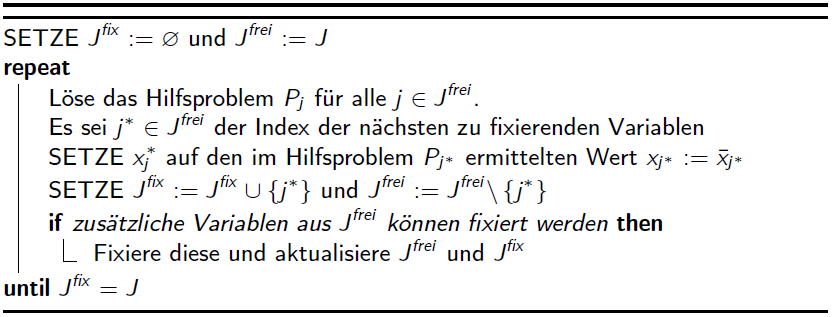
\includegraphics[scale =0.6]{AllgGreedy}
			\item Eröffnungsverfahren
			\item \hyperref[BPGreedy]{BPP-Greedy} und \hyperref[KPGreedy]{KP-Greedy}
			\item MST-Greedy Algorithmus: \\
				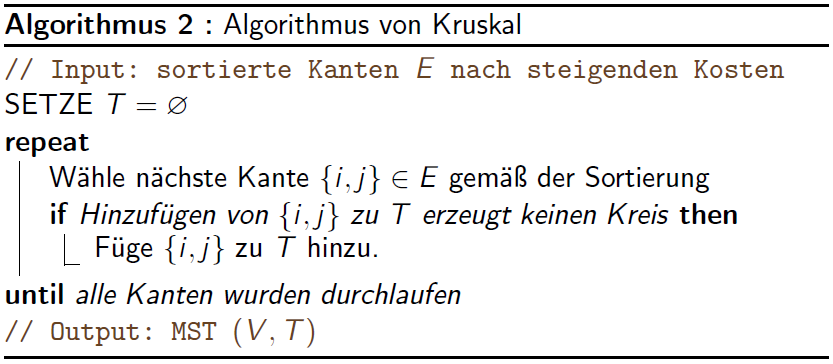
\includegraphics[scale=0.6]{KruskalGreedy}
			\item meinst \underline{nicht} optimal
			\item Nutzenmöglichkeit: \begin{enumerate}
					\item unzulässige Lösungen zulassen und mit Strafkosten versehen
					\item Wiederholen mit mod. Kosten/Koeffizienten/(Ersatz-)Problem
				\end{enumerate}
		\end{itemize}
	\section{3. Kapitel - Lösungsqualität und Approximation}
		\begin{itemize}
			\item\textbf{Performance-Verhältnis} \label{Performance Verhaeltnis}: Probleminstanz $P\in \Pi$, Heuristik \\ 
				$H \Rightarrow R_H(P)=\frac{z_H(P)}{z_{opt}(P)}$ 
			\item wenn Performance Verhältnis = 1 für alle Instanzen von $P$ $\Rightarrow$ exakter Opt.-Algo.
				\begin{itemize}
					\item Minimierungsproblem: $R_H(P) \ge 1$
					\item Maximierungsproblem: $R_H(P) \le 1$
				\end{itemize}
			\item \textbf{Performance Analysen}\label{Performance Analyse}:
				\begin{itemize}
					\item[worst-case:] schlechtestes Performance Verhältnis
					\item[average-case:] durchschnittliches Performance Verhältnis über \underline{alle} Instanzen, via Wahrscheinlichkeitsverteilung, Erwartungswert und Varianz
					\item[empirisch:] durchschnittliches Performance Verhältnis, maximale Abweichung und empirische Varianz über \underline{relevante} Instanzen
				\end{itemize}
			\item \textbf{$\epsilon$-Approximationsalgorithmus}\label{eApproxAlgo}: Für $\epsilon\ge 0$, Heuristik $H$. $H$ ist $\epsilon$-Approximationsalgorithmus gdw.
				\begin{itemize}
					\item $R_H \le 1- \epsilon$, für Minimierungsp.
					\item $R_H \ge 1- \epsilon$, für Maximierungsp.
				\end{itemize}
		\end{itemize}
	\section{4. Kapitel - Lokale Suche}
		\begin{itemize}
			\item Grundidee: geg. zulässige Lösung in eine andere bessere zulässige Lösung transformieren und rekursiv wiederholen
			\item \textbf{Nachbarschaft} \label{Nachbarschaft}: Abbildung $ \mathcal{N}:X\rightarrow Pot(X)$
			\item \textbf{verbessernder Nachbar} \label{verbessernder Nachbar}: zu min. Ziel-fkt $z$: $x'\in\mathcal{N}(X)$ mit $z(x')<z(x)$ heißt verbessernder Nachbar
			\item \hyperref[Nachbarschaft]{Nachbarschaften}, \hyperref[verbessernder Nachbar]{Nachbarn}
			\item Pseudocode:\\
				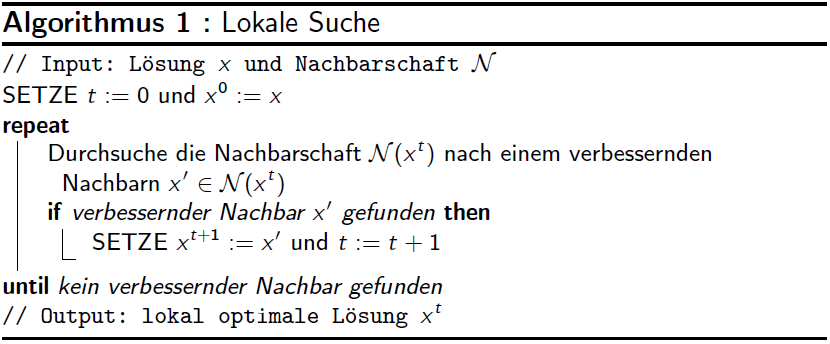
\includegraphics[scale=0.6]{LokaleSuche}
			\item Suchstrategien:
				\begin{itemize}
					\item[Erstensuche:] suche ersten \hyperref[verbessernder Nachbar]{verbessernden Nachbarn}
					\item[Bestensuche:] suche besten \hyperref[verbessernder Nachbar]{Nachbarn}
					\item[$l$-Erstensuche:] suche ersten $l$ \hyperref[verbessernder Nachbar]{verbessernde Nachbarn}
				\end{itemize}
			\item 2-Opt Nachbarschaft:
				\begin{itemize}
					\item Für (S)\hyperref[TSP]{TSP}: Entfernen von 2 nicht benachbarten Kanten und hinzufügen von zwei anderen
					\item $n$-Städte: $|\mathcal{N}_{2Opt}(X)|= \frac{n(n-3)}{2}$
				\end{itemize}
			\item \textbf{Nachbarschaftsgraph} \label{Nachbarschaftgraph}: $(X,A_\mathcal{N})$ mit $X$ alle zulässigen Lösungen, $(x,x')\in A_\mathcal{N}$, falls $x'\in\mathcal{N}(x)$
			\item \textbf{stark Zusammenhängend} \label{starker Zusammenhang}: Falls von jeder Lösung $x,y\in X$ ein Weg $\pi$ ex., sodass $\pi= x\dots y$
			\item \textbf{Transitionsgraph} \label{Transitionsgraph}: $(X,A_\mathcal{N}^{trans})$ mit $X$ alle zulässigen Lösungen, $(x,x')\in A_\mathcal{N}$, falls $x'$ ein \hyperref[verbessernder Nachbar]{verbessernder Nachbar} von $x$ ist
			\item \textbf{exakte Nachbarschaft}\label{exakte Nachbarschaft}: Wenn jedes lokale Optimum auch ein globales Optimum ist
			\item \textbf{Durchmesser einer Nachbarschaft}\label{Durchmesser}: max. Länge eines kürzesten Weges
			\item Wünschenswerte Eigenschaften:
				\begin{enumerate}
					\item \hyperref[starker Zusammenhang]{starker Zusammenhang}
					\item Symmetrie: $x\in\mathcal{N}(x') \Leftrightarrow x\in\mathcal{N}(x')$
					\item Effiziente Berechnung des Zielfunktionswertes.
					\item Effiziente Konstruktion von $\mathcal{N}$
					\item Effiziente Zulässigkeitsprüfung
					\item Effiziente Suche nach \hyperref[verbessernder Nachbar]{verbessernden Nachbarn}
				\end{enumerate}
			\item \textbf{Sequentielle Suche}\label{sequentielle Suche}:
				\begin{itemize}
					\item[Idee:] Lösche $(x,x')$ $\rightarrow$ Füge $(x',x'')$ hinzu $\rightarrow$ Lösche $(x'',x''')$ $\rightarrow$ \dots
					\item[In 2-Opt:] $t_1,t_2,t_3,t_4$, wobei $(t_1,t_2)$ und $(t_3,t_4)$ gelöscht und $(t_2,t_3)$ und $(t_1,t_4)$ hinzu gefügt wurden
					\item[$\Rightarrow$] für $g_1 = c_{t_1,t_2}-c_{t_2,t_3}$ und $g_2= c_{t_3,t_4}-c_{t_4,t_1}$ will man $g_1+g_2 > 0$ für Verbesserung
					\item[$\Rightarrow$] man genötigt $g_1 > 0$ und $g_1+g_2 > 0$ (einer muss $>0$ sein und wenn $g_1+g_2 > 0$ und $g_1\le0$ dann stimmt die Aussage für $g_1'=g_2$ und $g_2'=g_1$)
					\item Algorithmus:\\
						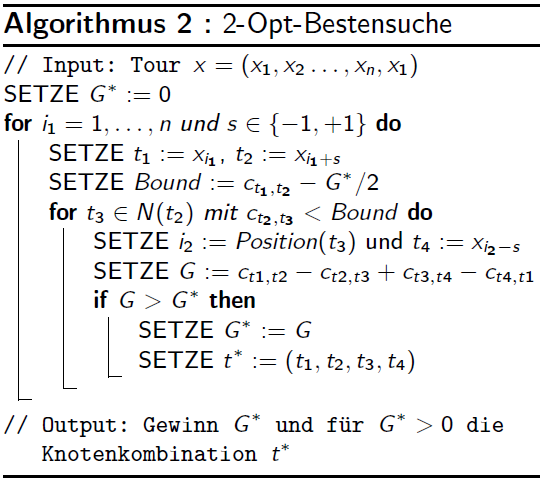
\includegraphics[scale=0.6]{SequentielleSucheAlgo}\\
						(Wichtig: \texttt{bound} fängt den symmetrischen Fall ab und bedeutet soviel wie: wir müssen bereits mit der ersten Löschung min. die Hälfte der Einsparung machen)
				\end{itemize}
		\end{itemize}
	\section{5. Kapitel - Metaheuristiken}
		\subsection{Einführung}
			\begin{itemize}
				\item Anwendungsbereich: exakte Verfahren nicht mehr anwendbar
				\item Eigenschaften: keine Optimalitätsgarantie, keine Aussage über Abweichung, akzeptable Lösungsgüte bei vernünftiger Laufzeit
				\item vom lokalen zum globalen Optima, via: 
					\begin{enumerate}
						\item Multi-Start
						\item Gedächtnis (Tabusuche) %TODO ref
						\item Randomisierung (Simulated Annealing)
						\item Pertubation (ILS, VND)
					\end{enumerate}
				\item "Def.": Strategien zum Steuern des Suchprozesses; unabhängig vom Problem; Konkretisierung $\Rightarrow$ Heuristik für spez. Optimierungsproblem
				\item Klassifikation ähnlich wie \hyperref[Heuristik]{hier} mit Erweiterung:
					\begin{itemize}
						\item Zufall: determinitistisch vs. zufallsgesteuert
						\item Gedächtnis: mit vs. ohne
						\item natur-analog: der Natur nachempfunden vs. künstlich
						\item Anzahl Lösungen: Nutzung einer Lösung vs. Population von Lösungen
					\end{itemize}
				\item Alternieren zwischen: Intensivierung und Diversifikation
				\item Effiziente Datenstrukturen/Subalgorithmen wichtiger Bestandteil
				\item Charakteristika:
					\begin{itemize}
						\item[Geschwindigkeit:]
							\begin{itemize}
								\item hängt von Planungsebene ab: strategisch vs. taktisch vs. operativ
								\item Echtzeitumgebung, dynamische Planung
								\item Interaktion
							\end{itemize}
						\item[Genauigkeit:]
							\begin{itemize}
								\item Abweichung von Optimallösung
								\item Konsistenz: lieber immer (nur) gut als mal sehr gut mal sehr schlecht
								\item[Problem:] Lösung durch genaues hinsehen schon verbesserbar
								\item Lieber gute Lösung + stetige Verbesserung sichtbar, als einfach finale Lösung
							\end{itemize}
						\item[Einfachheit:]
							\begin{itemize}
								\item Verständlichkeit von der Grundidee
								\item robust
								\item vernünftige Anzahl aussagekräftiger Parameter
							\end{itemize}
						\item[Flexibilität:]
							\begin{itemize}
								\item Anpassung durch weitere NB verringern nicht/kaum die Güte
							\end{itemize}
					\end{itemize}
			\end{itemize}

		\subsection{Iterierte Lokale Suche (ILS)}
			\subsubsection{Idee}
				Suche auf der Menge der lokalen Minima.
			\subsubsection{Algorithmus}
					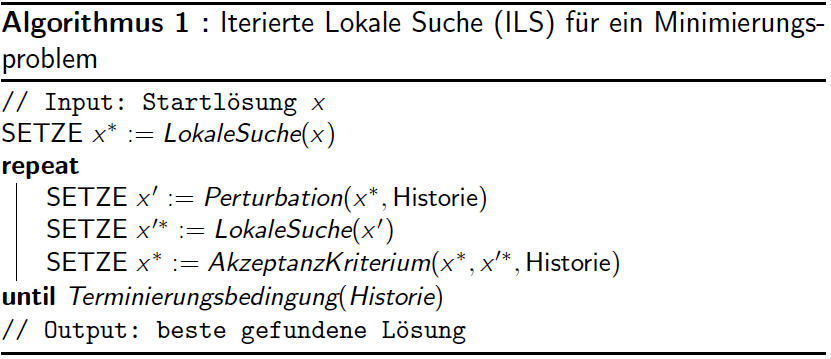
\includegraphics[scale=0.6]{ILS}\\
					\begin{enumerate}
						\item \texttt{LokaleSuche($x$)}: Verbesserung einer Lösung $x$ zu einem lokalen Optimum
						\item \texttt{Pertubation($x$,historie)}: verwirbelt eine Lösung
						\item \texttt{AkzeptanzKriterium($x$,$x'$,historie)}: akzeptiert $x'$ oder lässt $x$
					\end{enumerate}
			\subsubsection{Stärken}
				\begin{itemize}
					\item Gute Lösungsqualität mit einfacher Impl. (besser als zufällige Neustarts)
					\item konzeptuell einfach und modularer Aufbau
					\item Geschwindigkeit: besser als zufällige Neustarts
				\end{itemize}
			\subsubsection{Design}
				\begin{itemize}
					\item \textbf{Initiallösung}: Einfluss nimmt mit Länge des Suchverlaufs ab
					\item \textbf{Lokale Suche}: gründliche LS liefert meist bessere Ergebnisse
					\item \textbf{Pertubation}: 
						\begin{itemize}
							\setlength{\itemindent}{2cm}
							\item[zu schwach:] wenig Diversifikation
							\item[zu stark:] quasi zufällige Neustarts
							\item Abstimmung mit LS: Güte und Geschwindigkeit
						\end{itemize}
					\item \textbf{Akzeptanzkriterium}
						Oft basierend auf SA %TODO link zu Simulated Annealing
				\end{itemize}
		\subsection{Variable Neighborhood Descent (VND)}
			\subsubsection{Idee}
				Det. LS mit einer Folge von Nachbarschaften. Nur verbessernde Schritte und ende in lokalem Optimum bzgl. aller Nachbarschaften
			\subsubsection{Algorithmus}
				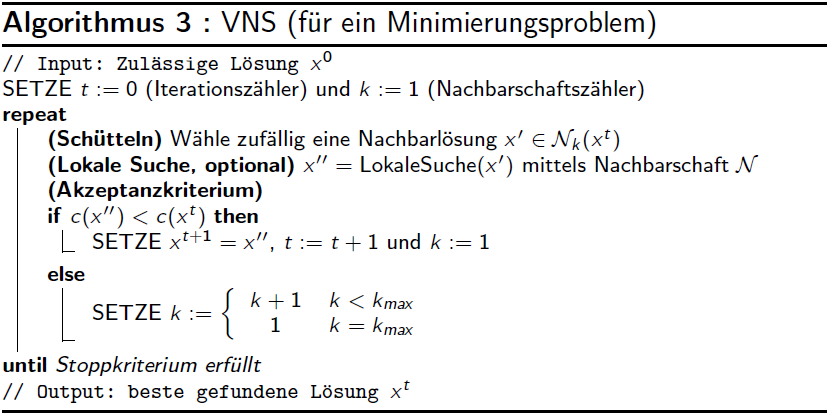
\includegraphics[scale=0.6]{VNS}
				\begin{itemize}
					\item[\texttt{$k_{max}=1$}] einfache ITS
					\item Bei Maximierung ersetze "<" durch ">"
%				\end{itemize}
%			\subsubsection{Bemerkung:}
%				\begin{itemize}
					\item Wenn bessere Lösung $x''$ gefunden wurde starte wieder bei $\mathcal{N}_1$
					\item Auswahl $x\in\mathcal{N}_k(x^t)$ sollte aufgrund einer Gleichverteilung erfolgen
				\end{itemize}
		\subsection{Tabu Search}\label{TabuSearch}
			\subsubsection{Idee}
				Gehe zur zur besten Nachbarlösung, welche mit den Tabu-Restriktionen vereinbar ist.
			\subsubsection{attributives vs. explizites Gedächtnis}
				\begin{tabular}{r|l l}
					Name & attributiv 		& explizit \\ \hline
					Speichern von: & einzelne Attribute einer Lösung(-sübergangs) & komplette Lösungen \\
					Typische Elemente: 	& \tabitem Vorhanden sein eines Obj. in einer Lösung 	& Verwaltung von Elite-Lös.\\
										& \tabitem Anzahl von Objekten							& \\
										& \tabitem Austausch von Objekten 						&  test\\
					Vorteil: 			& geringer Speicheraufwand								& kein Tabu für nicht \\
										&														& besuchte Lösungen\\
					Nachteil:			& mögl. tabu für nicht besuchte Lösung					& Speicheraufwendig
				\end{tabular}
			\subsubsection{Tabu Restriktionen}
				\begin{tabular}{ c c l}
					Nr. & Basis-Attribut & Tabu-Restriktion \\ \hline
					1 & \texttt{Inc(i)} & Verbietet Verringern von $x_i$ auf 0 \\
					2 & \texttt{Dec(j)} & Verbiete Erhöhen von $x_j$ auf 1 \\
					3 & \texttt{Inc(i)} und \texttt{Dec(j)} & Verbietet Nr. 1 und/oder 2 \\
					4 & \texttt{Swap(+i,-j)} & Verbietet Umkehrung \texttt{Swap(+j,-i)} \\
					5 & \texttt{c($x'$)-c($x$)} & Verbietet mit Ziel-fkt Änderung \texttt{c($x$)-c($x'$)} \\
					6 & \texttt{g($x'$)-g($x$)} & Verbietet Schritte mit Fkt Änderung \texttt{g($x$)-g($x'$)}
				\end{tabular}
				\begin{itemize}
					\item restriktivere Tabu-Restriktionen tabuisieren mehr Nachbarlösungen
					\item meist Versucht Inversion vom aktuellen zum vorherigen zu vermeiden
					\item Gedächtnis genutzt um Zyklen zu vermeiden
				\end{itemize}
			\subsubsection{Kurzzeitgedächtnis}	
				\begin{itemize}
					\item 
						\begin{enumerate}
							\item Füge neue Restriktionen in eine Liste der Länge $k$ ein
							\item Sind bereits alle $k$ Elemente genutzt lösche das "älteste" und füge die neuen hinzu
						\end{enumerate}
					\item zu kleines $k$ $\rightarrow$ höheres Zyklen-Risiko
					\item zu  großes $k$ $\rightarrow$ zu starke Einschränkung
				\end{itemize}
			\subsubsection{Anspruchskriterium}
				\begin{center}
					Wenn alle Nachbarlösungen tabu $\rightarrow$ wähle eine, welche tabu ist
				\end{center}
				\begin{tabular}{c l l}
					 & Anspruchskriterium & Bedeutung \\ \hline
					\tabitem & Anspruch bei Ermangelung & falls alle tabu, wähle die, die ''am wenigsten" tabu ist \\
					\tabitem & Anspruch durch Ziel- & falls der Zielfunktionswert besser ist als der bisher beste Wert\\
					 & funktionswert & ist die Lösung nicht mehr tabu. \\
					\tabitem & Anspruch durch & falls Restriktion gesetzt während Verbesserung und\\
					 & Suchrichtung &  tabuisierte erneut Verbesserung $\rightarrow$ hebe Restriktion auf\\
				\end{tabular}
			\subsubsection{Algorithmus}
				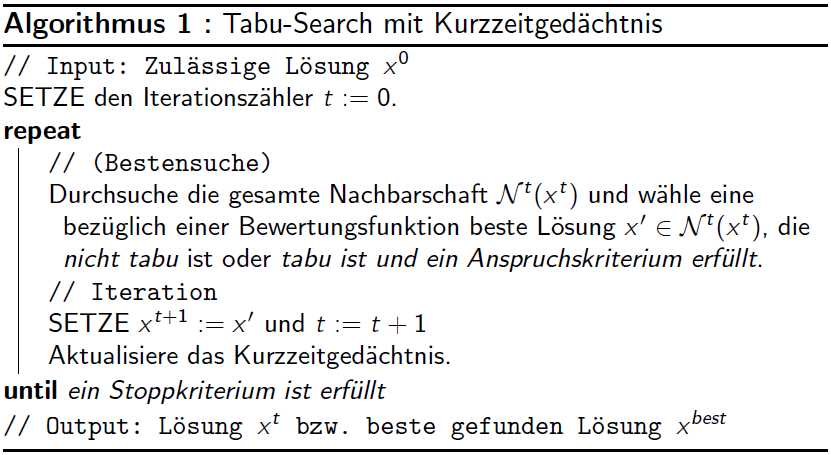
\includegraphics[scale=0.6]{TabuSearch}	
				\begin{itemize}
					\item als Lokale Suche meist Bestensuche $\rightarrow$ aggressive Suche
					\item Nachbarschaft kann im Laufe variiert werden
					\item beste Lösung immer explizit speichern
					\item Bewertungsfunktion kann von Zfkt. abweichen (Strafkosten, Einfluss auf Struktur)
				\end{itemize}
				
	\section{Large Neighboorhood Search (LNS)}
		Alternative Namen: Ruin and Recreate, Fix and Optimize
		\subsection{Idee}
			Graduelle Verbesserung einer Lösung durch Destroy- (entfernen eines Teils) und Repair- (bauen entfernte anders wieder auf) Operatoren.
			
		\subsection{Algorithmus}
			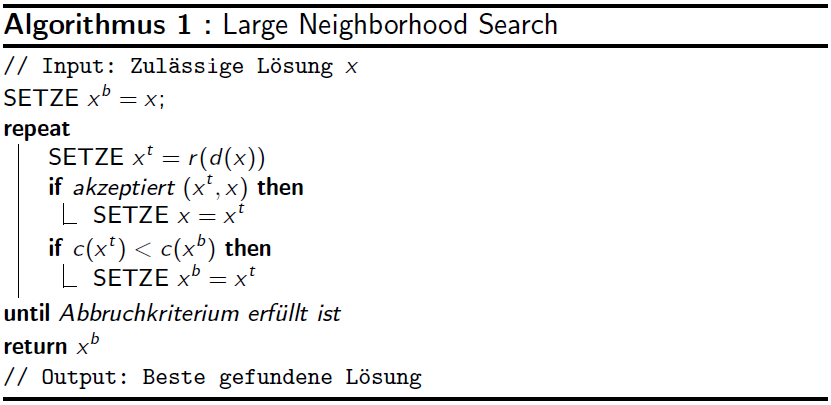
\includegraphics[scale=0.6]{LNS}
			\begin{itemize}
				\item Zufall: versch. Teile der Lösung zerstören $\rightarrow$ Diversifikation
				\item Zerstörungsgrad:
					\begin{itemize}
						\item zu gering $\rightarrow$ keine Exploration des Lösungsraums
						\item zu hoch $\rightarrow$ zeitaufwendig und wenig erfolgversprechend
					\end{itemize}
			\end{itemize}
		\subsection{Destroy-Operatoren}
			\begin{tabular}{l l l}
				Name & Beschreibung & Effekt \\ \hline
				Random Destroy & Entferen zufällige Elemente & Diversifikation \\
				Worst/Critial Destroy & Entferne teuersten Elemente & Intensivierung \\
				Related Destroy & Entferne leicht austauschbare Elemente & Intensivierung \\
				Small Removal & Entferne Variablen mit geringen Koeff. & Intensivierung \\
				History-Based Destroy & Entferne Elemente die Teil einer & Diversifikation\\
				& schlechter Lösungen waren & 				
			\end{tabular}
		\subsection{Repair-Operatoren}
			\begin{itemize}
				\item \hyperref[greedy]{Greedy Heuristiken}: iterativ bestmögliche Wahl \\
					Problem: Wahlmöglichkeiten in späteren Iterationen
				\item Regret Heuristiken: maximale Differenz zwischen bester Einfügemöglichkeit und $k$-bester
				\item Relaxierte exakte Verfahren: Beschleunigung
				\item Exakte Verfahren: schnell gute Lösungen, keine Diversifikation
				\item Lokale Suche
			\end{itemize}
	\section{Adaptive Neighborhood Search (ALNS)}
		\subsection{Idee}
			Anwenden von mehreren gewichteten Destroy- und Repair-Operatoren, mit dynamischer Gewichtsanpassung basierend auf vorherigen Iterationen
		\subsubsection{Algorithmus}
			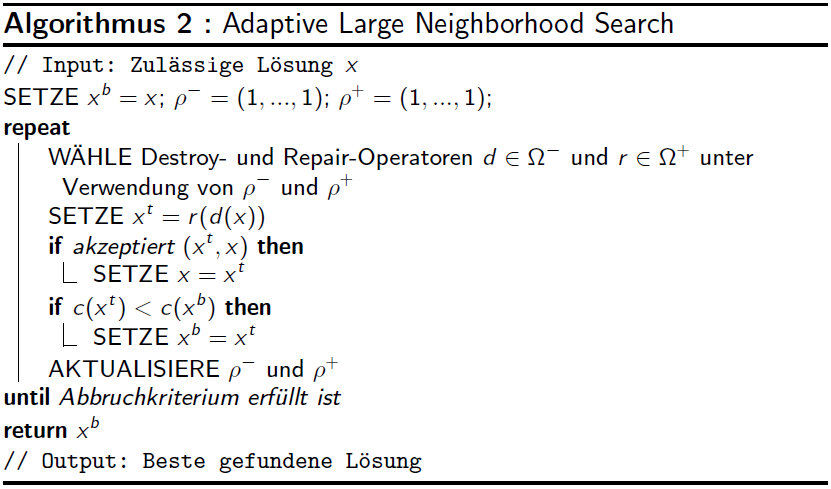
\includegraphics[scale=0.6]{ALNS}
			\begin{itemize}
				\item robust durch adaptiven Mechanismus
				\item keine explizite Nachbarschafts Auswahl nötig
			\end{itemize}
\end{document}
























